\documentclass[tikz,border=8pt]{standalone}
% Shared look for every TikZ diagram. Load with % Shared look for every TikZ diagram. Load with % Shared look for every TikZ diagram. Load with \input{../../tools/tikz-style.tex}
\usepackage[T1]{fontenc}
\usepackage{lmodern}
\renewcommand{\sfdefault}{lmr}  % diagrams use the same serif as the text
\usetikzlibrary{arrows.meta, positioning, shapes.geometric, calc, fit, backgrounds}
\definecolor{cblue}{HTML}{4C78A8}
\definecolor{corange}{HTML}{F58518}
\definecolor{cgreen}{HTML}{54A24B}
\definecolor{cred}{HTML}{E45756}
\definecolor{cpurple}{HTML}{B279A2}
\definecolor{cgrey}{HTML}{6B6B6B}
\tikzset{
  every picture/.style={font=\sffamily, line width=1.2pt},
  box/.style={draw=#1, fill=#1!12, rounded corners=4pt, align=center, inner sep=7pt, minimum height=1.1cm},
  box/.default=cgrey,
  arrow/.style={-{Stealth[length=3mm]}, draw=cgrey, line width=1.4pt},
  title/.style={font=\sffamily\bfseries\Large},
  note/.style={font=\sffamily\small, text=cgrey, align=center},
}
\AtBeginDocument{\hyphenpenalty=10000 \exhyphenpenalty=10000}

\usepackage[T1]{fontenc}
\usepackage{lmodern}
\renewcommand{\sfdefault}{lmr}  % diagrams use the same serif as the text
\usetikzlibrary{arrows.meta, positioning, shapes.geometric, calc, fit, backgrounds}
\definecolor{cblue}{HTML}{4C78A8}
\definecolor{corange}{HTML}{F58518}
\definecolor{cgreen}{HTML}{54A24B}
\definecolor{cred}{HTML}{E45756}
\definecolor{cpurple}{HTML}{B279A2}
\definecolor{cgrey}{HTML}{6B6B6B}
\tikzset{
  every picture/.style={font=\sffamily, line width=1.2pt},
  box/.style={draw=#1, fill=#1!12, rounded corners=4pt, align=center, inner sep=7pt, minimum height=1.1cm},
  box/.default=cgrey,
  arrow/.style={-{Stealth[length=3mm]}, draw=cgrey, line width=1.4pt},
  title/.style={font=\sffamily\bfseries\Large},
  note/.style={font=\sffamily\small, text=cgrey, align=center},
}
\AtBeginDocument{\hyphenpenalty=10000 \exhyphenpenalty=10000}

\usepackage[T1]{fontenc}
\usepackage{lmodern}
\renewcommand{\sfdefault}{lmr}  % diagrams use the same serif as the text
\usetikzlibrary{arrows.meta, positioning, shapes.geometric, calc, fit, backgrounds}
\definecolor{cblue}{HTML}{4C78A8}
\definecolor{corange}{HTML}{F58518}
\definecolor{cgreen}{HTML}{54A24B}
\definecolor{cred}{HTML}{E45756}
\definecolor{cpurple}{HTML}{B279A2}
\definecolor{cgrey}{HTML}{6B6B6B}
\tikzset{
  every picture/.style={font=\sffamily, line width=1.2pt},
  box/.style={draw=#1, fill=#1!12, rounded corners=4pt, align=center, inner sep=7pt, minimum height=1.1cm},
  box/.default=cgrey,
  arrow/.style={-{Stealth[length=3mm]}, draw=cgrey, line width=1.4pt},
  title/.style={font=\sffamily\bfseries\Large},
  note/.style={font=\sffamily\small, text=cgrey, align=center},
}
\AtBeginDocument{\hyphenpenalty=10000 \exhyphenpenalty=10000}

\begin{document}
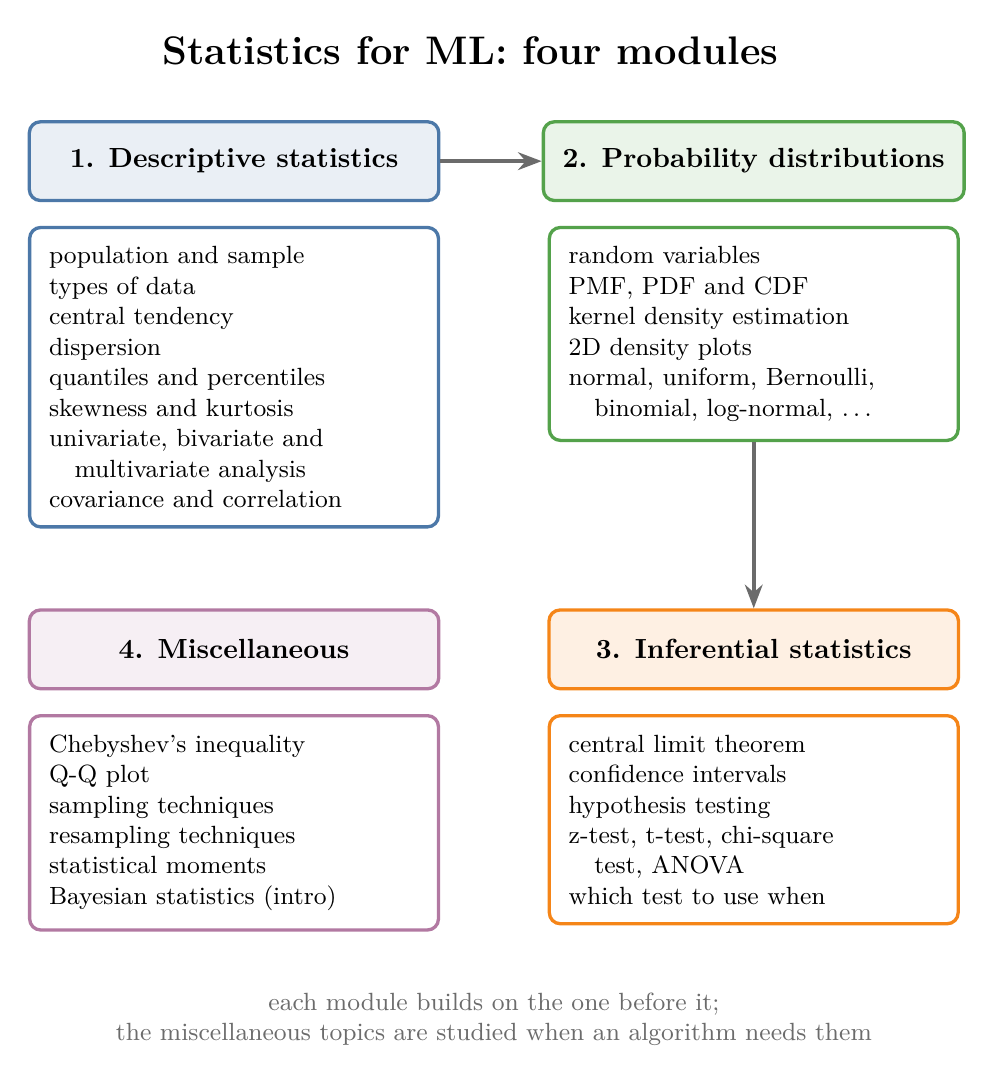
\begin{tikzpicture}[
  mod/.style={box=#1, font=\sffamily\bfseries, minimum width=5.2cm, minimum height=1cm},
  topics/.style={draw=#1, fill=white, rounded corners=4pt, align=left, inner sep=7pt, text width=4.7cm, font=\sffamily\small},
]
  \node[title] at (3,1.4) {Statistics for ML: four modules};

  \node[mod=cblue] (d) at (0,0) {1. Descriptive statistics};
  \node[topics=cblue, below=0.3cm of d] (dt) {population and sample\\ types of data\\ central tendency\\ dispersion\\ quantiles and percentiles\\ skewness and kurtosis\\ univariate, bivariate and\\ \quad multivariate analysis\\ covariance and correlation};

  \node[mod=cgreen] (p) at (6.6,0) {2. Probability distributions};
  \node[topics=cgreen, below=0.3cm of p] (pt) {random variables\\ PMF, PDF and CDF\\ kernel density estimation\\ 2D density plots\\ normal, uniform, Bernoulli,\\ \quad binomial, log-normal, \dots};

  \node[mod=corange] (i) at (6.6,-6.2) {3. Inferential statistics};
  \node[topics=corange, below=0.3cm of i] (it) {central limit theorem\\ confidence intervals\\ hypothesis testing\\ z-test, t-test, chi-square\\ \quad test, ANOVA\\ which test to use when};

  \node[mod=cpurple] (m) at (0,-6.2) {4. Miscellaneous};
  \node[topics=cpurple, below=0.3cm of m] (mt) {Chebyshev's inequality\\ Q-Q plot\\ sampling techniques\\ resampling techniques\\ statistical moments\\ Bayesian statistics (intro)};

  \draw[arrow] (d.east) -- (p.west);
  \draw[arrow] (pt.south) -- (i.north);
  \node[note] at (3.3,-10.9) {each module builds on the one before it;\\ the miscellaneous topics are studied when an algorithm needs them};
\end{tikzpicture}
\end{document}
